\frame{
\frametitle{Variability of pulG filaments as seen by EM}
\begin{tabular}{m{.5\textwidth}|m{.5\textwidth}}
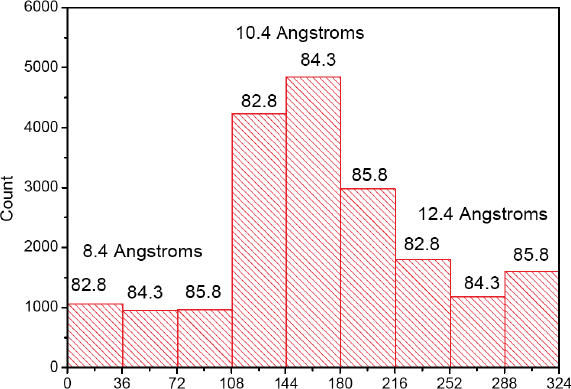
\includegraphics[width=0.5\textwidth]{figures/emdist.png}&
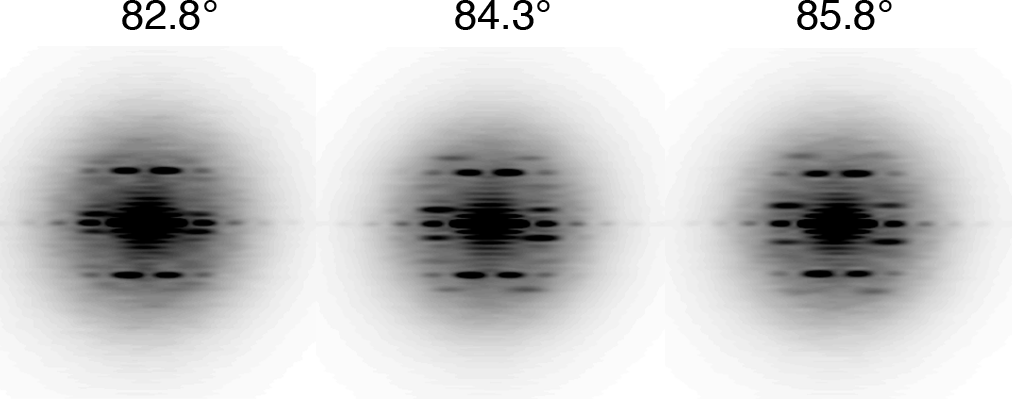
\includegraphics[width=0.5\textwidth]{figures/powerspectra.png}\\
\end{tabular}
\begin{block}{Conformational sampling}
... during the multistage procedure a twist angle was randomly chosen between 81 and 88 degrees with uniform probability. 3901 models were obtained and clustered with SOM.\\
3D coordinates of one monomer and symmetry information were used as input vectors for the SOM.
\end{block}
\footnotesize{From Nivaskumar, Bouvier et al. 2013}
}
